\par\addvspace{12pt}\Needspace{9\baselineskip}

\section{二次曲线的化简、分类与几何结构}

% ITEM: quadratic-example-012
\solutionitem{quadratic-example-012}{例4.12}
通过旋转与平移化简方程\(5x^2-6xy+5y^2-8x-8y=0\)，写出所用的新旧坐标关系，并画出曲线的示意图。
\solutionanswer
取\(U=(x+y-4)/\sqrt2,V=(y-x)/\sqrt2\)，即平移中心到\((2,2)\)后将轴旋转\(45^\circ\)，方程化为\(2U^2+8V^2=16\)，即\(U^2/8+V^2/2=1\)。半轴为\(2\sqrt2,\sqrt2\)，长轴沿\((1,1)\)。
\begin{center}
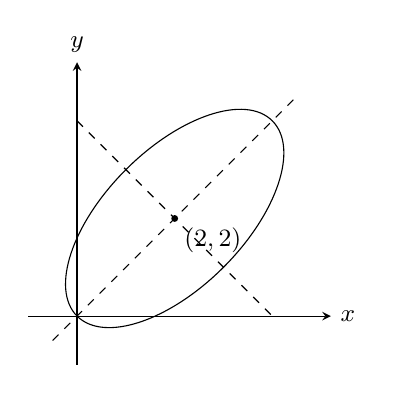
\begin{tikzpicture}[scale=.62,>=stealth,font=\small]
\draw[->] (-1,0)--(5.2,0) node[right]{$x$};
\draw[->] (0,-1)--(0,5.2) node[above]{$y$};
\draw[shift={(2,2)},rotate=45] (0,0) ellipse(2.828cm and 1.414cm);
\draw[dashed] (-.5,-.5)--(4.5,4.5) (0,4)--(4,0);
\fill (2,2) circle(2pt) node[below right]{$(2,2)$};
\end{tikzpicture}
\end{center}


% ITEM: quadratic-example-013
\solutionitem{quadratic-example-013}{例4.13}
分别求\(x^2+2xy+2y^2-2x=0\)与\(x^2-2xy+y^2-x-y=0\)的中心；若不存在，说明原因。选择适当坐标，将两个方程分别化简。
\solutionanswer
第一条曲线中心满足\(x+y=1,x+2y=0\)，故为\((2,-1)\)。取\(u=x+y-1,v=y+1\)，方程成为\(u^2+v^2=2\)。第二条的中心条件要求\(2(x-y)=1\)及\(2(y-x)=1\)，互相矛盾，故无中心。取\(u=(x-y)/\sqrt2,v=(x+y)/\sqrt2\)，方程化为\(2u^2=\sqrt2v\)。


% ITEM: quadratic-example-014
\solutionitem{quadratic-example-014}{例4.14 *}
对例4.12中的方程，求二次部分的特征值与单位特征向量，利用矩阵计算中心及化简后的完整方程，并与旋转、配方的结果比较。
\solutionanswer
二次部分矩阵\(H=\left(\begin{smallmatrix}5&-3\\-3&5\end{smallmatrix}\right)\)的特征值为\(2,8\)，对应单位特征向量分别为\((1,1)/\sqrt2\)和\((-1,1)/\sqrt2\)。记\(L=(-8,-8)^T\)，由\(2HC+L=0\)得中心\(C=-H^{-1}L/2=(2,2)^T\)。平移\(X=C+\xi\)后，常数为\(C^THC+L^TC=-16\)。
取以上单位特征向量为列组成正交矩阵\(S\)，再令\(\xi=S(U,V)^T\)，有\(S^THS=\operatorname{diag}(2,8)\)，所以完整方程为\(2U^2+8V^2=16\)。对应\(U=(x+y-4)/\sqrt2,V=(y-x)/\sqrt2\)，与旋转、配方所得坐标及方程完全相同。


% ITEM: quadratic-example-015
\solutionitem{quadratic-example-015}{例4.15}
讨论\(x^2+2txy+y^2=1\)随实参数\(t\)变化时的曲线类型，并在\(t=0,1,2\)时分别写出简化后的方程。
\solutionanswer
令\(u=(x+y)/\sqrt2,v=(y-x)/\sqrt2\)，得到\((1+t)u^2+(1-t)v^2=1\)。\(|t|<1\)为椭圆（\(t=0\)为圆），\(|t|=1\)为两平行直线，\(|t|>1\)为双曲线。\(t=0,1,2\)依次给出\(u^2+v^2=1,2u^2=1,3u^2-v^2=1\)。


% ITEM: quadratic-example-016
\solutionitem{quadratic-example-016}{例4.16}
分别构造判别式相同的三个二次方程，使它们表示椭圆、单点与空集；再构造两个二次方程，使它们分别表示抛物线与两条平行直线，且都有\(\Delta=0\)。
\solutionanswer
\(x^2+y^2=1\)与\(x^2+y^2=-1\)都有\(\Delta=-4\)，前者为实圆，后者为空集。\(y^2=x\)、\(x^2=y\)都是\(\Delta=0\)的抛物线；\(y^2=1\)、\(x^2=4\)都是\(\Delta=0\)的两平行直线。可见判别式不能单独决定完整方程的类型。


% ITEM: quadratic-exercise-07-01
\solutionitem{quadratic-exercise-07-01}{习题4.7（1）}
将\(x^2+2xy+y^2-2x+2y=0\)化为不含交叉项和常数项的方程，写出坐标关系。
\par
\solutionanswer
取旋转坐标\(x=(u-v)/\sqrt2,\ y=(u+v)/\sqrt2\)，即新轴分别沿原坐标的\((1,1)\)、\((-1,1)\)方向。则
\[(x+y)^2-2x+2y=2u^2+2\sqrt2v=0.\]
令\(U=u,V=v\)，化简方程为\(U^2+\sqrt2V=0\)，已无交叉项和常数项。该代换的坐标关系即上述\(x,y\)表达式。


% ITEM: quadratic-exercise-07-02
\solutionitem{quadratic-exercise-07-02}{习题4.7（2）}
将\(3x^2+2xy+3y^2-8=0\)化简，并求曲线上点到原点距离的最大值与最小值。
\par
\solutionanswer
取\(u=(x+y)/\sqrt2,v=(y-x)/\sqrt2\)，方程成为\(4u^2+2v^2=8\)，即\(u^2/2+v^2/4=1\)。旋转保距，故到原点距离的最大值为\(2\)，最小值为\(\sqrt2\)。


% ITEM: quadratic-exercise-07-03
\solutionitem{quadratic-exercise-07-03}{习题4.7（3）}
对\(x^2+2xy+y^2-4x-4y+3=0\)，求式\textup{(4.48)}的全部解，并说明这些点与曲线的关系。
\par

\par\smallskip\noindent 正文所引关系为：
\begin{equation*}
\begin{cases}
        2Ah+Bk+D=0 ,\\
        Bh+2Ck+E=0
    \end{cases}
\end{equation*}
\solutionanswer
方程的中心条件两式均为\(2h+2k-4=0\)，故全部解为直线\(h+k=2\)。原方程可写成
\[(x+y)^2-4(x+y)+3=0,\quad (x+y-1)(x+y-3)=0,\]
即两条平行线\(x+y=1,3\)。每个满足\(h+k=2\)的点均在两平行线等距的中线上；关于该点中心对称会互换两条线，因此都是曲线的对称中心。不存在唯一中心。


% ITEM: quadratic-exercise-07-04
\solutionitem{quadratic-exercise-07-04}{习题4.7（4）}
对例4.12中的方程，分别采用先旋转后平移、先求中心再旋转的顺序化简，比较所得坐标关系与方程。
\par
\solutionanswer
先旋转时取\(u=(x+y)/\sqrt2,v=(y-x)/\sqrt2\)，方程为\(2(u-2\sqrt2)^2+8v^2=16\)，再令\(U=u-2\sqrt2,V=v\)。先平移时取\(\xi=x-2,\eta=y-2\)，再令\(U=(\xi+\eta)/\sqrt2,V=(\eta-\xi)/\sqrt2\)。两条路线最终完全相同，均为\(U^2/8+V^2/2=1\)。


% ITEM: quadratic-exercise-07-05
\solutionitem{quadratic-exercise-07-05}{习题4.7（5）}
分别判断\(x^2+y^2=0\)、\(x^2-y^2=0\)、\(x^2=4\)、\((x-y-1)^2=0\)、\(x^2+y^2=-1\)、\(x^2=-1\)的图形，并比较后两个方程。
\par
\solutionanswer
依次是原点、两条相交直线\(x=\pm y\)、两条平行直线\(x=\pm2\)、重直线\(x-y=1\)、空集、空集。后两式实解集均为空，但二次部分分别有两个和一个平方项，方程类型不同。


% ITEM: quadratic-exercise-07-06
\solutionitem{quadratic-exercise-07-06}{习题4.7（6）}
讨论\(x^2+y^2-2x+4y+t=0\)随\(t\)变化时的曲线类型。
\par
\solutionanswer
配方得
\[(x-1)^2+(y+2)^2=5-t.\]
当\(t<5\)时为圆，圆心\((1,-2)\)、半径\(\sqrt{5-t}\)；当\(t=5\)时仅有点\((1,-2)\)；当\(t>5\)时无实点。


% ITEM: quadratic-exercise-07-07
\solutionitem{quadratic-exercise-07-07}{习题4.7（7）}
对\(x^2-2xy+y^2+dx+ey+f=0\)，按\(d+e\)是否为零分类；当\(d+e=0\)时，再讨论\(f\)的影响。
\par
\solutionanswer
令\(u=(x-y)/\sqrt2,v=(x+y)/\sqrt2\)，得到\(2u^2+(d-e)u/\sqrt2+(d+e)v/\sqrt2+f=0\)。\(d+e\ne0\)时可配方为抛物线。若\(e=-d\)，原式为\((x-y+d/2)^2=d^2/4-f\)，所以\(f<d^2/4\)时为两平行直线，等号时为重直线，\(f>d^2/4\)时为空集。


% ITEM: quadratic-exercise-07-08
\solutionitem{quadratic-exercise-07-08}{习题4.7（8）}
求经过\((0,0)\)、\((1,0)\)、\((0,1)\)、\((1,1)\)、\((2,3)\)的二次曲线方程，并判断类型。
\par
\solutionanswer
代入前四点得\(F=B=0,D=-A,E=-C\)，最后一点给出\(A=-3C\)。取\(C=1\)，得到\(-3x^2+y^2+3x-y=0\)。令\(X=x-1/2,Y=y-1/2\)，则\(3X^2-Y^2=1/2\)，是实双曲线。


% ITEM: quadratic-exercise-07-09
\solutionitem{quadratic-exercise-07-09}{习题4.7（9）}
若五个给定点中有三点共线，一定不能唯一确定二次曲线吗？考察其中恰有三点共线、另两点均不在该直线上的情形。
\par
\solutionanswer
可以唯一确定，方程只差非零常数倍。存在性来自六个系数所满足的五个齐次一次条件：消元至多确定五个主元，仍有非零解。若有两条不同的二次曲线通过五点，将方程分别限制到连接其中两点的直线上。限制式均非零，否则其余三点须共线。两个二次式有相同两根，故可取线性组合使限制式恒为零。该组合含此直线为因子，其余三点又迫使另一个一次因子经过它们，与不三点共线矛盾；故两方程必成比例。

恰有三点共线时，二次方程限制到该直线有三个不同根，必须含该直线为因子；其余两点确定另一直线，故唯一曲线是这两条直线的并。


% ITEM: quadratic-exercise-07-10
\solutionitem{quadratic-exercise-07-10}{习题4.7（10）}
将\(x^2+4xy+5y^2=1\)通过可逆一次坐标代换化为单位圆方程。这个代换是否保持长度与夹角？再用旋转化简，与前一种方法比较。
\par
\solutionanswer
由\(x^2+4xy+5y^2=(x+2y)^2+y^2\)，取\(u=x+2y,v=y\)，即成为单位圆。它不保长保角，例如两个标准单位向量的像为\((1,0),(2,1)\)。若先旋转，取旋转角\(-\pi/8\)可消去交叉项，得到\((3-2\sqrt2)r^2+(3+2\sqrt2)s^2=1\)，再沿两轴伸缩化圆。前者直接配方，后者保留了主轴方向与长度信息。


% ITEM: quadratic-exercise-07-11
\solutionitem{quadratic-exercise-07-11}{习题4.7（11）}
证明非退化实二次曲线至多有一个对称中心，并说明两条平行直线组成的图形为什么可以有无穷多个中心。
\par
\solutionanswer
若有两个不同中心，连续做两次中心对称就是一个非零平移。选曲线上一点，反复平移得到同一直线上的无穷多曲线点。二次方程限制到这条直线便恒为零，因而包含一个直线因子，曲线退化，矛盾。两条平行直线则不同：中间平行线上的每一点作为中心，都会将两原直线互换，因此有无穷多个中心。


% ITEM: quadratic-exercise-07-12
\solutionitem{quadratic-exercise-07-12}{习题4.7（12）}
求以\((1,-1)\)为中心，且经过\((3,-1)\)、\((1,0)\)、\((2,0)\)的二次曲线方程，并判断类型。
\par
\solutionanswer
令\(X=x-1,Y=y+1\)，中心条件使方程没有一次项。代入三个新坐标\((2,0),(0,1),(1,1)\)，得\(4A+F=C+F=A+B+C+F=0\)。取\(A=1\)，方程为\(X^2-XY+4Y^2=4\)。二次式等于\((X-Y/2)^2+15Y^2/4\)，所以是实椭圆。


% ITEM: quadratic-exercise-07-13
\solutionitem{quadratic-exercise-07-13}{习题4.7（13） *}
求\(q(x,y)=2x^2+2xy+2y^2\)的特征方向与标准形，并用标准形证明\(q\)正定。
\par
\solutionanswer
二次型矩阵为\(H=\begin{bmatrix}2&1\\1&2\end{bmatrix}\)。方向\((1,1)\)、\((1,-1)\)分别是特征方向，对应特征值\(3\)、\(1\)。取正交单位坐标\(u=(x+y)/\sqrt2\)、\(v=(x-y)/\sqrt2\)，则标准形为
\[
q=3u^2+v^2.
\]
两个平方项系数都为正，所以除\((u,v)=(0,0)\)外\(q>0\)，即\(q\)正定。


% ITEM: quadratic-exercise-07-14
\solutionitem{quadratic-exercise-07-14}{习题4.7（14） *}
设实二阶对称矩阵\(H\)的两个特征值分别为\(\lambda_1,\lambda_2\)。证明\(\lambda_1+\lambda_2=A+C\)、\(\lambda_1\lambda_2=AC-B^2/4\)，并说明正定性与这两个特征值的关系。
\par
\solutionanswer
展开特征方程
\[
\det(H-\lambda I)=\lambda^2-(A+C)\lambda+AC-B^2/4=0.
\]
由根与系数的关系即得两式。正交标准形为\(\lambda_1u^2+\lambda_2v^2\)，所以正定当且仅当两个特征值都为正。


% ITEM: quadratic-exercise-07-15
\solutionitem{quadratic-exercise-07-15}{习题4.7（15） *}
设\(H\)不可逆而\(2Ht+L=0\)有解。证明解集是一条直线，并在\(q(x,y)=(x+y)^2\)上举例说明。
\par
\solutionanswer
二次曲线的二次部分非零，故奇异\(H\)的秩为\(1\)，核是一维。任取特解\(t_0\)，全部解为\(t_0+\ker H\)，所以是一条直线。例如\((x+y)^2-4x-4y+3=0\)的中心条件为\(h+k=2\)，其全部解就是一条直线。


% ITEM: quadratic-example-017
\solutionitem{quadratic-example-017}{例4.17 *}
分别求\(x^2+4y^2=4\)、\(x^2-4y^2=4\)、\(y=x^2\)的\(H\)与\(M\)的秩。给出前两条曲线在复数范围内的一个可逆坐标代换，并说明为什么不能用同类代换将第三条曲线变成前两条曲线。
\solutionanswer
三式的\((\operatorname{rank}H,\operatorname{rank}M)\)依次为\((2,3),(2,3),(1,3)\)。完整齐次矩阵分别为
\[
 \operatorname{diag}(1,4,-4),\qquad
 \operatorname{diag}(1,-4,-4),\qquad
 \begin{pmatrix}1&0&0\\0&0&-1/2\\0&-1/2&0\end{pmatrix}.
\]
前两条曲线之间可作复可逆代换\(x=u,y=iv\)，将\(x^2+4y^2=4\)变为\(u^2-4v^2=4\)。反向代换为\(u=x,v=-iy\)。
但可逆仿射代换的二次部分按\(H\mapsto S^THS\)变化，秩保持不变。抛物线的\(H\)秩为\(1\)，前两条曲线的\(H\)秩为\(2\)，因此即使允许复数系数，也不能用同类仿射代换把抛物线变成前两条曲线。三条曲线的完整矩阵秩同为\(3\)，所以这里只看\(M\)的秩还不够。


% ITEM: quadratic-exercise-08-01
\solutionitem{quadratic-exercise-08-01}{习题4.8（1） *}
将\(2u^2+3v^2\)、\(2u^2-3v^2\)、\(2u^2\)分别通过实可逆线性代换化为系数只含\(1,-1,0\)的形式，记录各自的正负系数个数与秩。
\par
\solutionanswer
分别作可逆伸缩：
\[
U=\sqrt2\,u,\quad V=\sqrt3\,v
\]
把\(2u^2+3v^2\)化为\(U^2+V^2\)；
\[
U=\sqrt2\,u,\quad V=\sqrt3\,v
\]
把\(2u^2-3v^2\)化为\(U^2-V^2\)；对\(2u^2\)取\(U=\sqrt2\,u\)、\(V=v\)，化为\(U^2+0V^2\)。相应正、负系数个数及秩依次为\((2,0),2\)；\((1,1),2\)；\((1,0),1\)。


% ITEM: quadratic-exercise-08-02
\solutionitem{quadratic-exercise-08-02}{习题4.8（2） *}
比较\(x^2+y^2+1=0\)、\(x^2+y^2=0\)、\(x^2+1=0\)的\(H\)与\(M\)的秩，并在复数范围内判断能否分解为一次因子的乘积。
\par
\solutionanswer
三式的\((\operatorname{rank}H,\operatorname{rank}M)\)依次为\((2,3),(2,2),(1,2)\)。后两式分别分解为\((x+iy)(x-iy)=0\)、\((x+i)(x-i)=0\)。第一式不能分成两个一次因子：若能，其完整齐次矩阵至多为两个列向量的对称乘积之和，秩至多\(2\)，与\(M=I_3\)矛盾。


% ITEM: quadratic-exercise-08-03
\solutionitem{quadratic-exercise-08-03}{习题4.8（3） *}
证明\(u^2+v^2\)与\(u^2-v^2\)在实数范围内不合同，在复数范围内却合同。
\par
\solutionanswer
实数范围内，\(u^2+v^2\)在每个非零向量处为正，可逆实代换保持这一性质；\(u^2-v^2\)却可取负值，故不合同。复数范围取\(u=r,v=is\)，前式即为\(r^2-s^2\)，代换可逆，故合同。


% ITEM: quadratic-exercise-08-04
\solutionitem{quadratic-exercise-08-04}{习题4.8（4） *}
若一个二次方程整体乘以\(-1\)，其矩阵的正负系数个数如何变化？曲线是否变化？据此说明分类二次型与分类方程的实解集有什么区别。
\par
\solutionanswer
正、负系数个数交换，秩不变；实解集不变。因此用符号结构分类方程的实解集时，还应把整体非零倍数表示的同一方程识别起来。


% ITEM: quadratic-exercise-08-05
\solutionitem{quadratic-exercise-08-05}{习题4.8（5） *}
比较\(x^2+y^2=1\)与\(x^2-y^2=1\)的\(H\)、\(M\)的秩。仅凭这两个秩能否判断它们仿射等价？再利用二次部分的符号结构作出判断。
\par
\solutionanswer
两曲线的\(H\)秩均为\(2\)，\(M\)秩均为\(3\)，单凭秩无法区分。前者二次部分正定，后者不定；即使允许方程整体乘负数，定号与不定仍不能混同，因此不实仿射等价。


% ITEM: quadratic-exercise-08-06
\solutionitem{quadratic-exercise-08-06}{习题4.8（6） *}
代换\(x=u\)、\(y=iv\)将复曲线\(x^2+y^2=1\)化为\(u^2-v^2=1\)。原实圆上哪些点对应实双曲线上的点？据此解释复化后等价与实仿射等价的区别。
\par
\solutionanswer
代换\(x=u\)、\(y=iv\)后，\(x^2+y^2=1\)成为\(u^2-v^2=1\)。若原点\((x,y)\)在实圆上且对应的\((u,v)\)也为实数，则\(x=u\)实，而\(y=iv\)要实只能有\(v=0\)，即\(y=0\)。圆上因此只有\((x,y)=(1,0),(-1,0)\)，分别对应双曲线上的\((u,v)=(1,0),(-1,0)\)。这说明复化后的可逆代换建立的是复点之间的对应；除这两点外，实圆的点像不在实平面中，故复仿射等价不意味着实仿射等价。


% ITEM: quadratic-exercise-08-07
\solutionitem{quadratic-exercise-08-07}{习题4.8（7） *}
对方程\(x^2+y^2-2tx+1=0\)，讨论实参数\(t\)变化时完整齐次矩阵\(M\)的秩与实图形的类型，并说明代数退化发生在何时。
\par
\solutionanswer
有\(M=\begin{bmatrix}1&0&-t\\0&1&0\\-t&0&1\end{bmatrix}\)，其行列式为\(1-t^2\)。故\(t=\pm1\)时秩为\(2\)，其余时候为\(3\)。配方得\((x-t)^2+y^2=t^2-1\)，所以\(|t|>1\)为实圆，\(|t|=1\)为单点，\(|t|<1\)为空集；代数退化只发生在\(t=\pm1\)。


% ITEM: quadratic-example-018
\solutionitem{quadratic-example-018}{例4.18}
对椭圆\(x^2/4+y^2=1\)，求斜率为\(1\)的弦所对应的直径，并求与这条直径共轭的直径。比较两条直径的夹角与圆中相应的结论。
\solutionanswer
弦方向为\(d=(1,1)\)，中点满足\(x/4+y=0\)，故共轭直径方向可取\(e=(4,-1)\)。将\(rd\)、\(se\)代入椭圆，分别得\(r=\pm2/\sqrt5,s=\pm1/\sqrt5\)，因此两条直径长度为\(4\sqrt{2/5}\)、\(2\sqrt{17/5}\)。两方向夹角余弦为\(3/\sqrt{34}\)，一般不垂直；圆中的共轭直径则始终垂直。


% ITEM: quadratic-exercise-09-01
\solutionitem{quadratic-exercise-09-01}{习题4.9（1）}
求椭圆\(x^2/9+y^2/4=1\)的水平弦与竖直弦分别对应的直径。
\par
\solutionanswer
水平弦端点为\((x,y),(-x,y)\)，中点在\(x=0\)上；竖直弦的中点同理在\(y=0\)上。因此对应的直径直线分别为\(x=0,y=0\)，相应直径线段分别连接\((0,\pm2)\)、\((\pm3,0)\)。


% ITEM: quadratic-exercise-09-02
\solutionitem{quadratic-exercise-09-02}{习题4.9（2）}
求抛物线\(y=x^2\)上斜率为\(2\)的弦中点的轨迹，明确轨迹与整条直径的区别。
\par
\solutionanswer
设端点为\((1+h,(1+h)^2)\)、\((1-h,(1-h)^2)\)，\(h\ne0\)。它们的连线斜率为\(2\)，中点为\((1,1+h^2)\)。所以中点轨迹恰为\(x=1,y>1\)，是整条直径直线\(x=1\)的一部分。


% ITEM: quadratic-exercise-09-03
\solutionitem{quadratic-exercise-09-03}{习题4.9（3）}
对椭圆\(x^2/a^2+y^2/b^2=1\)，推导两条斜率均存在的共轭直径之间的斜率关系。对双曲线\(x^2/a^2-y^2/b^2=1\)作同样的研究。
\par
\solutionanswer
将斜率为\(m\)的平行弦代入方程，比较两根的平均值，椭圆中点满足\(x/a^2+my/b^2=0\)。该直径斜率\(n=-b^2/(a^2m)\)，故\(mn=-b^2/a^2\)。双曲线同理给出\(x/a^2-my/b^2=0\)，于是\(mn=b^2/a^2\)。这些关系针对题设中两斜率均存在的情形。


% ITEM: quadratic-exercise-09-04
\solutionitem{quadratic-exercise-09-04}{习题4.9（4）}
将圆作变换\(x'=2x+y\)、\(y'=y\)。证明原圆的一对垂直直径变为像曲线的一对共轭直径，并说明一般的仿射变换为什么保持共轭直径关系。
\par
\solutionanswer
原圆中，一方向的平行弦中点都在垂直于它的直径上。仿射变换保持中点、直线和平行性，所以像中的这一平行弦族中点仍在另一条像直径上，两像直径共轭。论证只用了仿射性质，对任意可逆仿射变换均成立。


% ITEM: quadratic-exercise-09-05
\solutionitem{quadratic-exercise-09-05}{习题4.9（5）}
椭圆的任意两条互相垂直的直径是否一定共轭？分别讨论圆与非圆椭圆。
\par
\solutionanswer
圆中成立。非圆椭圆中不一定：设两垂直方向为\((\cos\theta,\sin\theta)\)、\((-\sin\theta,\cos\theta)\)，共轭条件化为\((a^2-b^2)\sin\theta\cos\theta=0\)。\(a\ne b\)时只有两条主轴方向满足，其他垂直直径一般不共轭。


% ITEM: quadratic-exercise-09-06
\solutionitem{quadratic-exercise-09-06}{习题4.9（6）}
求椭圆\(x^2/4+y^2=1\)上以\((1,1/2)\)为中点的弦所在直线，并求弦长。
\par
\solutionanswer
以\(M=(1,1/2)\)为中点写两端点为\(M\pm(u,v)\)。代入椭圆方程相减得\(u+2v=0\)，相加得\(u^2/4+v^2=1/2\)，故\((u,v)=\pm(1,-1/2)\)。弦直线为\(x+2y=2\)，端点\((2,0),(0,1)\)，弦长\(\sqrt5\)。


% ITEM: quadratic-exercise-09-07
\solutionitem{quadratic-exercise-09-07}{习题4.9（7）}
求双曲线\(xy=1\)上以\((2,1)\)为中点的弦所在直线及两个端点。若中点改为\((1,1)\)，这样的弦是否存在？说明理由。
\par
\solutionanswer
写端点为\((2,1)\pm(u,v)\)，两乘积等于\(1\)给出\(u+2v=0,uv=-1\)，故\((u,v)=\pm(\sqrt2,-1/\sqrt2)\)。直线为\(x+2y=4\)，端点为\((2\pm\sqrt2,1\mp1/\sqrt2)\)。若中点为\((1,1)\)，同理得\(u+v=uv=0\)，只能有\(u=v=0\)，不能构成非退化弦。


% ITEM: quadratic-example-019
\solutionitem{quadratic-example-019}{例4.19 *}
设\(q(x,y)=2x^2+2xy+2y^2\)。求\(d=(1,0)\)的共轭方向，再求与自身的共轭方向垂直的所有方向，并联系\(q=1\)的对称轴解释结果。
\solutionanswer
\(b(d,e)=2e_1+e_2\)，故共轭方向可取\((1,-2)\)。由\(q=(x+y)^2+x^2+y^2>0\)，非零方向不能满足\(b(d,d)=0\)，所以不存在自身共轭方向。几何上\(q=1\)为椭圆，没有由零方向给出的渐近线。


% ITEM: quadratic-exercise-10-01
\solutionitem{quadratic-exercise-10-01}{习题4.10（1） *}
对\(q(x,y)=x^2-y^2\)，分别求\((1,0)\)、\((1,2)\)、\((1,1)\)在\(b\)下的共轭方向。最后一种情形与前两种有什么不同？
\par
\solutionanswer
共轭条件是\(d_1e_1-d_2e_2=0\)。三个给定方向对应的共轭方向依次可取\((0,1),(2,1),(1,1)\)。最后一个与自身共轭，因其二次型值为零；前两个与各自的共轭方向线性无关。


% ITEM: quadratic-exercise-10-02
\solutionitem{quadratic-exercise-10-02}{习题4.10（2） *}
设\(H\)可逆、\(d\ne0\)，且\(q(d)\ne0\)。证明\(d\)与其共轭方向线性无关。若\(q(d)=0\)，共轭方向又是什么？
\par
\solutionanswer
\(H\)可逆保证\(e\mapsto d^THe\)为非零线性式，故其零空间是一条方向线。若\(q(d)\ne0\)，\(d\)不在该线上，因此与共轭方向线性无关；若\(q(d)=0\)，\(d\)就在此方向线上，故共轭方向与自身重合。


% ITEM: quadratic-exercise-10-03
\solutionitem{quadratic-exercise-10-03}{习题4.10（3） *}
设\(S\)可逆，证明\(q'(u)=q(Su)\)的共轭方向经\(S\)映射后，成为\(q\)的共轭方向。结合弦中点说明这一结论的几何意义。
\par
\solutionanswer
由极化或直接展开，\(b'(u,v)=b(Su,Sv)\)，所以新型的共轭方向映为原型的共轭方向。弦中点由仿射变换映为像弦中点，这与共轭直径的几何保持性一致。


% ITEM: quadratic-exercise-10-04
\solutionitem{quadratic-exercise-10-04}{习题4.10（4） *}
对\(x^2+2xy+2y^2-2x=0\)，写出\(H\)、\(L\)，利用双线性型求水平弦所对应的直径，并验证它经过曲线的中心。
\par
\solutionanswer
\(H=\begin{bmatrix}1&1\\1&2\end{bmatrix},L=(-2,0)^T\)。水平弦的中点条件为\((HM+L/2)\cdot(1,0)=0\)，即直径\(x+y=1\)。中心方程解为\((2,-1)\)，确在该直线上。


% ITEM: quadratic-exercise-10-05
\solutionitem{quadratic-exercise-10-05}{习题4.10（5） *}
设二元二次型\(q\)不定且非退化，\(d,e\)线性无关并满足\(b(d,e)=0\)。以\(d,e\)为基写出\(q\)的表达式，并证明\(q(d)q(e)<0\)。
\par
\solutionanswer
任意向量唯一写成\(sd+te\)，且\(q(sd+te)=s^2q(d)+t^2q(e)\)。非退化保证两个系数非零；不定性又保证能取正负值，因此两个系数异号，\(q(d)q(e)<0\)。


% ITEM: quadratic-example-020
\solutionitem{quadratic-example-020}{例4.20}
求\(x^2-2xy-3y^2-2x+10y-7=0\)的中心与两条渐近线，并求两条渐近线的夹角。
\solutionanswer
中心条件给出\((2,1)\)。令\(u=x-2,v=y-1\)，方程成为\((u-3v)(u+v)=4\)，故渐近线为\(x-3y+1=0,x+y-3=0\)。两线夹角的余弦为\(1/\sqrt5\)，故夹角为\(\arccos(1/\sqrt5)\)。


% ITEM: quadratic-exercise-11-01
\solutionitem{quadratic-exercise-11-01}{习题4.11（1）}
求\((x-1)^2/4-(y+2)^2/9=1\)的中心与渐近线。
\par
\solutionanswer
中心为\((1,-2)\)。将平移后的二次部分令为零，得渐近线\(y+2=\pm(3/2)(x-1)\)。


% ITEM: quadratic-exercise-11-02
\solutionitem{quadratic-exercise-11-02}{习题4.11（2）}
求\(xy-2x+y-3=0\)的渐近线，并以平移后的坐标说明曲线各部分相对渐近线的位置。
\par
\solutionanswer
写成\((x+1)(y-2)=1\)，故中心为\((-1,2)\)，渐近线为\(x=-1,y=2\)。令\(u=x+1,v=y-2\)，则\(uv=1>0\)，两分支分别位于新坐标的第一、第三象限。


% ITEM: quadratic-exercise-11-03
\solutionitem{quadratic-exercise-11-03}{习题4.11（3）}
设双曲线的渐近线为\(y=2x\)与\(y=-2x\)，且经过\((1,1)\)。求它的方程。若只给出两条渐近线，方程是否唯一确定？
\par
\solutionanswer
方程应为\((y-2x)(y+2x)=k\)，代入\((1,1)\)得\(k=-3\)，故\(4x^2-y^2=3\)。只给渐近线时，任意\(k\ne0\)均给出一个成员，不能唯一确定双曲线。


% ITEM: quadratic-exercise-11-04
\solutionitem{quadratic-exercise-11-04}{习题4.11（4）}
证明抛物线\(y=x^2\)没有直线渐近线。先考察竖直线，再对任意非竖直线使用点到直线的距离公式。
\par
\solutionanswer
曲线上点为\((t,t^2)\)，无穷远处必有\(|t|\to\infty\)。它到\(ax+by+c=0\)的距离为\(|at+bt^2+c|/\sqrt{a^2+b^2}\)。若\(b=0\)，距离随\(|t|\)发散；若\(b\ne0\)，二次项使距离发散。因此没有直线渐近线。


% ITEM: quadratic-exercise-11-05
\solutionitem{quadratic-exercise-11-05}{习题4.11（5）}
设双曲线在中心坐标下的方程为\(q(X)=1\)。证明任一条渐近线与双曲线没有公共点，并说明平行于渐近线的直线为什么至多有一个交点。
\par
\solutionanswer
渐近线上的点满足\(q=0\)，故不能同时满足\(q=1\)。平行于渐近方向\(d\)的直线写为\(P+td\)，因\(q(d)=0\)，限制式为\(q(P)+2t b(P,d)=1\)，是一次关系，至多有一个解。若一次系数也为零，由非退化性和二维共轭关系得\(P\parallel d\)，该直线就是渐近线且无解；其余平行线恰有一个交点。


% ITEM: quadratic-exercise-11-06
\solutionitem{quadratic-exercise-11-06}{习题4.11（6）}
求\((x-y)(2x+y)=3\)的两条渐近线。设曲线上一点到两条渐近线的距离分别为\(d_1,d_2\)，证明\(d_1d_2\)为常数，并求其值。
\par
\solutionanswer
中心为原点，渐近线为\(x-y=0,2x+y=0\)。两距离乘积为\(|(x-y)(2x+y)|/(\sqrt2\sqrt5)=3/\sqrt{10}\)，与点的位置无关。


% ITEM: quadratic-exercise-11-07
\solutionitem{quadratic-exercise-11-07}{习题4.11（7）}
讨论\(xy+tx+y+1=0\)随实参数\(t\)变化时的曲线类型。非退化时，求中心与渐近线；退化时，写出两个一次因子，并联系此前的渐近线解释。
\par
\solutionanswer
改写为\((x+1)(y+t)=t-1\)。\(t\ne1\)时为非退化双曲线，中心\((-1,-t)\)，渐近线\(x=-1,y=-t\)；\(t=1\)时分解为\((x+1)(y+1)=0\)，原来的两渐近线成为曲线本身的两个直线分量。


% ITEM: quadratic-exercise-11-08
\solutionitem{quadratic-exercise-11-08}{习题4.11（8）}
证明双曲线\(x^2/a^2-y^2/b^2=1\)除\(y=\pm(b/a)x\)外没有其他直线渐近线。可从曲线上点到一般直线\(lx+my+n=0\)的距离出发。
\par
\solutionanswer
沿\(x\to+\infty\)的两分支，\(y=\pm(b/a)\sqrt{x^2-a^2}\)，且\(\sqrt{x^2-a^2}-x\to0\)。要使\(lx+my+n\to0\)，必先有\(l\pm mb/a=0\)，再有\(n=0\)。因此只能得到\(y=\pm(b/a)x\)；左侧两无穷分支给出相同结论。这两条直线确使距离趋于零。
\par
